\lab{Wave Phenomena}{Wave Phenomena}
\label{lab:waveeqn}

\section*{Advection Equation}
The advection equation (or transport equation) is given by $u_t + s u_x = 0$, where $s$ is a nonzero constant.
Consider the Cauchy problem
\begin{align*}
	& u_t + su_x = 0, \quad -\infty < x < \infty,\\\
	& u(x,0) = f(x).
\end{align*}
The function $f(x)$ may be thought of as an initial wave or signal.
The general solution of this initial boundary value problem is $u(x,t) = f(x-st)$ (check this!).
The solution $u(x,t)$ is a travelling wave that takes the signal $f(x)$ and moves it along at a constant speed $s$ - to the right if $s > 0$, and to the left if $s < 0$.

\section*{Wave Equation}
Many different wave phenomena can be described using a hyperbolic PDE called the wave equation.
These wave phenomena occur in fields such as electromagnetics, fluid dynamics, and acoustics.
This equation is given by
\begin{align}
	u_{tt} &= s^2 \triangle u.
\end{align}
The 1D equation can be derived in the context of many physical models; a common derivation describes the motion of a string vibrating in a plane.
Another nice derivation uses Hooke's law from the theory of elasticity.

After making the change of variables $(\xi,\eta) = (x-st, x + st)$ and using the chain rule, we find that the 1D wave equation $u_{tt} = s^2 u_{xx}$ is equivalent to $u_{\xi \eta} = 0$.
The general solution of this last equation is
\[u(\xi, \eta) = F(\xi) + G(\eta)\]
for some scalar functions $F$ and $G$.
In $(x,t)$ coordinates the solution is
\[u(x,t) = F(x-st) + G(x+st)\]
Thus the general solution of the wave equation is the sum of two parts: one is a signal travelling to the right with constant speed $|s|$, and the other is a signal travelling to the left with speed $|s|$.

The wave equation is usually seen in the context of an initial boundary value problem.
This takes the form
\begin{align*}
	u_{tt} &= s^2 u_{xx}, \quad 0 < x < l, \quad t > 0,\\
	u(0,t) &= u(l,t) = 0, \\
	u(x,0) &= f(x),\\
	u_t(x,0) &= g(x).
\end{align*}

\subsection*{Numerical solution of the wave equation}
We look to approximate $u(x,t)$ on a grid of points $(x_j,t_m)_{j=0,m=0}^{J,M}$.
Denote the approximation to $u(x_j,t_m)$ by $U_{j}^{m}$.
Recall that the centered approximations in space and time are
\begin{align*}
D_{tt} U_{j}^{m} = \frac{U_{j}^{m+1} -2 U_{j}^{m} + U_{j}^{m-1}}{(\triangle t)^2} ,\\
D_{xx} U_{j}^{m} = \frac{U_{j+1}^{m} -2 U_{j}^{m} + U_{j-1}^{m}}{(\triangle x)^2} .
\end{align*}

The resulting method is given by
\begin{align*}
	&\frac{U_{j}^{m+1} -2 U_{j}^{m} + U_{j}^{m-1}}{(\triangle t)^2} = s^2 \frac{U_{j+1}^{m} -2 U_{j}^{m} + U_{j-1}^{m}}{(\triangle x)^2}, \\
	&U_{j}^{m+1} =  - U_{j}^{m-1} + 2 (1-\lambda^2) U_{j}^{m} + \lambda ^2 (U_{j+1}^{m} + U_{j-1}^{m}),
\end{align*}
where $ \lambda  =  s(\triangle t)/(\triangle x)$.
This method may be written in matrix form as
\[U^{m+1} = AU^{m} - U^{m-1} \]
where
\[A =
\left[\begin{array}{cccc}2(1-\lambda^2) & \lambda^2 &  &  \\ \lambda^2 & 2(1-\lambda^2) & \lambda^2 &  \\ \ddots & \ddots & \ddots &  \\ & \lambda^2 & 2(1-\lambda^2) & \lambda^2 \\  &  & \lambda^2 & 2(1-\lambda^2)\end{array}\right]\]
and
\[U^m = \left[\begin{array}{c}U_{1}^{m} \\U_{2}^{m} \\\vdots \\U_{J-1}^{m}\end{array}\right]\]

In the matrix equation above, we have already used the boundary conditions to determine that $U_{0}^{m} = U_{J}^{m} = 0$ at each time $t_m$.
Note that, to obtain the approximation $U_{j}^{m+1}$ of $u(x_j,t_{m+1})$, the method uses the value of the approximation at \emph{the previous two time steps}.
We can find the solution for the first two time steps by using the initial conditions.
Using the initial conditions directly gives an approximation at $t = t_0 = 0:$
\[U_{j}^{0} = f(x_j), \quad 1 \leq j \leq J-1\]

To obtain an approximation at the second time step, we consider the Taylor expansion
\begin{align*}
	u(x_j,t_1) &= u(x_j, 0) + u_t(x_j,0) \triangle t + u_{tt}(x_j,0) \frac{\triangle t^2}{2} + u_{ttt}(x_j,t_1^*) \frac{\triangle t^3}{6}.
\end{align*}
Recalling that the solution $u(x,t)$ satisfies the wave equation, we substitute in expressions from our initial conditions:
\begin{align*}
	u(x_j,t_1) &= u(x_j, 0) +  g(x_j) \triangle t+ s^2 f''(x_j)\frac{\triangle t^2}{2} +  u_{ttt}(x_j,t_1^*) \frac{\triangle t^3}{6}.
\end{align*}
Ignoring the third order term, we obtain a second order approximation for the second time step:
\[U_{j}^{1}= U_{j}^{0} + g(x_j) \triangle t+ s^2 f''(x_j) \frac{\triangle t^2}{2}, \quad 1 \leq j \leq J-1\]
or if $f$ is not readily differentiable,
\[U_{j}^{1}= U_{j}^{0} + g(x_j) \triangle t+ \frac{\lambda^2}{2} (U^0_{j-1} -2 U^0_j + U^0_{j+1})\]
This method is conditionally stable; the CFL condition is that $\lambda \leq 1$.

\begin{problem}
\label{prob:prob1}
Consider the initial boundary value problem
\begin{align*}
	u_{tt} &= u_{xx}, \\
	u(0,t) &= u(1,t) = 0, \\
	u(x,0) &= \sin(2 \pi x),\\
	u_t(x,0) &= 0.
\end{align*}
Numerically approximate the solution $u(x,t)$ for $t \in \left[0,.5\right]$.
Use $J=50$ subintervals in the $x$ dimension and $M=50$ subintervals in the $t$ dimension.
Animate the results.
Compare your results with the analytic solution $u(x,t) = \sin{(2 \pi x)} \cos{(2 \pi t)}$.
This function is known as a standing wave.
See Figure \ref{fig:prob1}.

\begin{figure}[H]
\centering
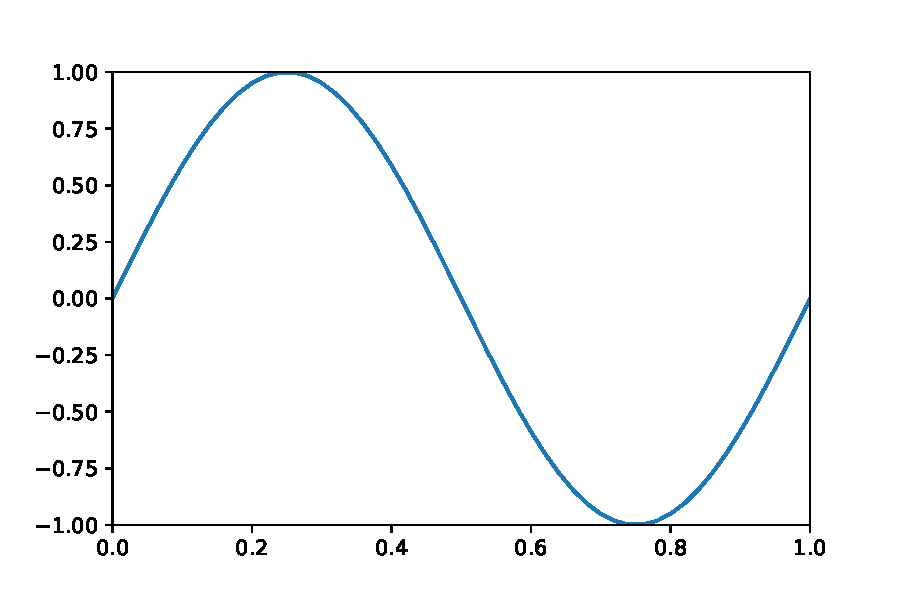
\includegraphics[width=\textwidth]{prob1.pdf}
\caption{$u(x,t=0)$.}
\label{fig:prob1}
\end{figure}
\end{problem}

\begin{problem}
\label{prob:prob2}
Consider the initial boundary value problem
\begin{align*}
	u_{tt} &= u_{xx}, \\
	u(0,t) &= u(1,t) = 0, \\
	u(x,0) &= .2e^{-m^2(x-1/2)^2}\\
	u_t(x,0) &= .4m^2(x-1/2)e^{-m^2(x-1/2)^2}.
\end{align*}
The solution of this problem is a Gaussian pulse.
It travels to the right at a constant speed.
This solution models, for example, a wave pulse in a stretched string.
Note that the fixed boundary conditions reflect the pulse back when it meets the boundary.

Numerically approximate the solution $u(x,t)$ for $t \in \left[0, 1\right]$.
Set $m=20$.
Use 200 subintervals in space and 220 in time, and animate your results.
Then use 200 subintervals in space and 180 in time, and animate your results.
Note that the stability condition is not satisfied for the second mesh.
See \ref{fig:prob2}.

\begin{figure}[H]
\centering
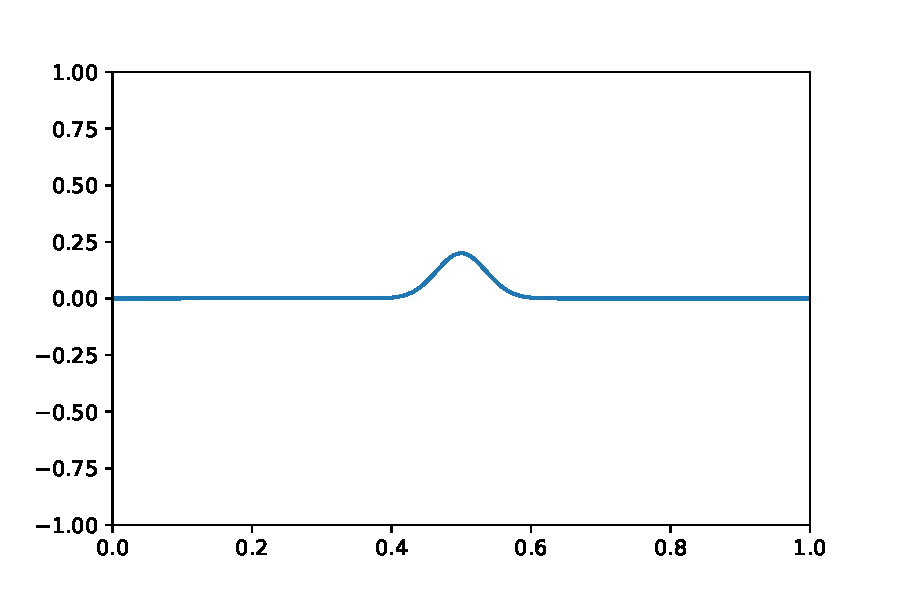
\includegraphics[width=\textwidth]{prob2.pdf}
\caption{$u(x,t=0)$.}
\label{fig:prob2}
\end{figure}
\end{problem}

\begin{problem}
\label{prob:prob3}
Consider the initial boundary value problem
\begin{align*}
	u_{tt} &= u_{xx}, \\
	u(0,t) &= u(1,t) = 0, \\
	u(x,0) &= .2e^{-m^2(x-1/2)^2}\\
	u_t(x,0) &= 0.
\end{align*}
The initial condition separates into two smaller, slower-moving pulses, one travelling to the right and the other to the left.
This solution models, for example, a plucked guitar string

Numerically approximate the solution $u(x,t)$ for $t \in \left[0,2\right]$.
Set $m=20$.
Use 200 subintervals in space and 440 in time, and animate your results.
It is rather easy to see that the solution to this problem is the sum of two travelling waves, one travelling to the left and the other to the right, as described earlier.
\end{problem}

\begin{problem}
\label{prob:prob4}
Consider the initial boundary value problem
\begin{align*}
	u_{tt} &= u_{xx}, \\
	u(0,t) &= u(1,t) = 0, \\
	u(x,0) &= \begin{cases} 1/3 & \text{if } 5/11 < x < 6/11,\\
	0 & \text{otherwise}
	\end{cases}\\
	u_t(x,0) &= 0.
\end{align*}

Numerically approximate the solution $u(x,t)$ for $t \in \left[0, 2\right]$.
Use 200 subintervals in space and 440 in time, and animate your results.
Even though the method is second order and stable for this discretization, since the initial condition is discontinuous there are large dispersive errors.
See Figure \ref{fig:prob4}.

%\begin{figure}[H]
%\centering
%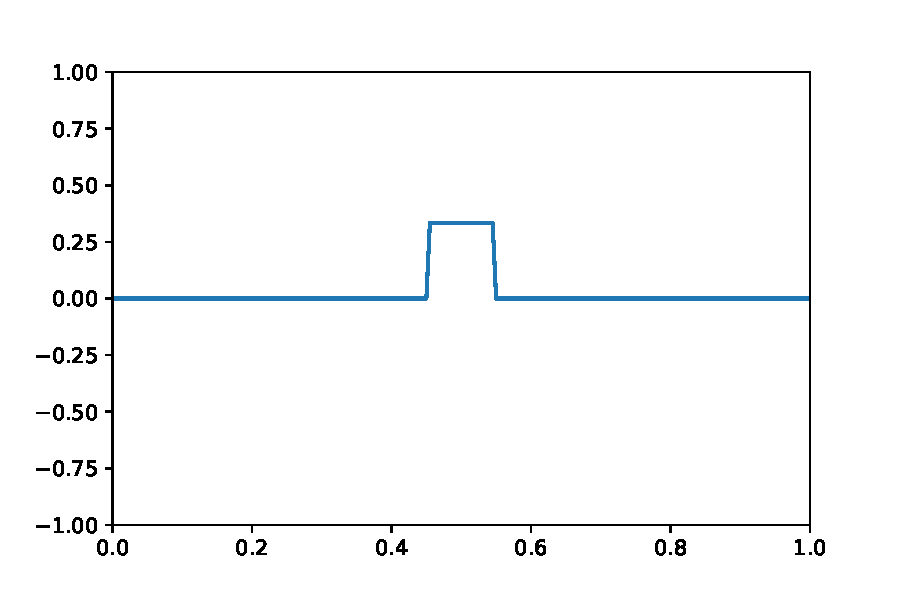
\includegraphics[width=\textwidth]{prob4.pdf}
%\caption{$u(x,t=0)$.}
%\label{fig:prob4}
%\end{figure}
%\end{problem}

\begin{figure}[H]
\centering
\begin{subfigure}{.49\textwidth}
\centering
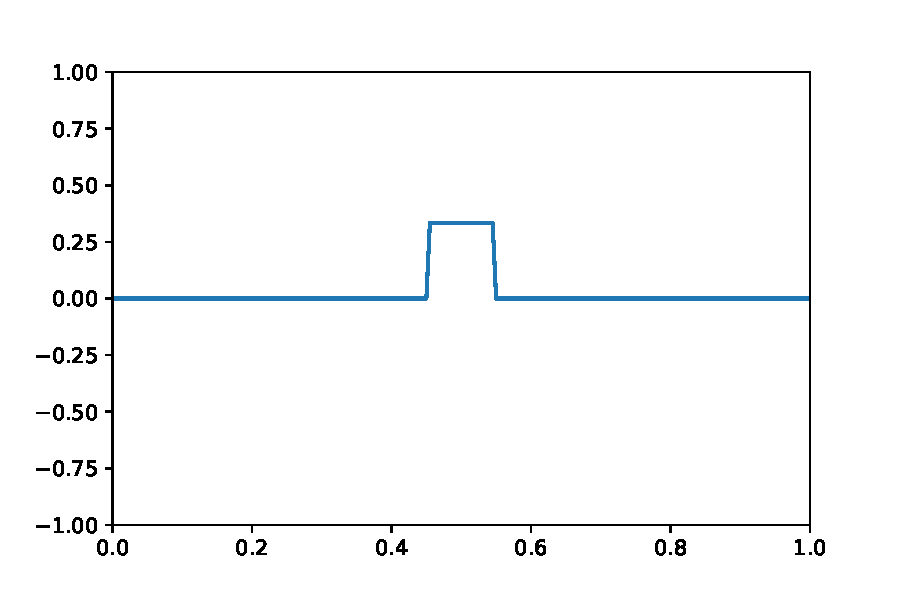
\includegraphics[width=\linewidth]{prob4.pdf}
\caption{$u(x,t=0)$.}
\end{subfigure}
%
\begin{subfigure}{.49\textwidth}
\centering
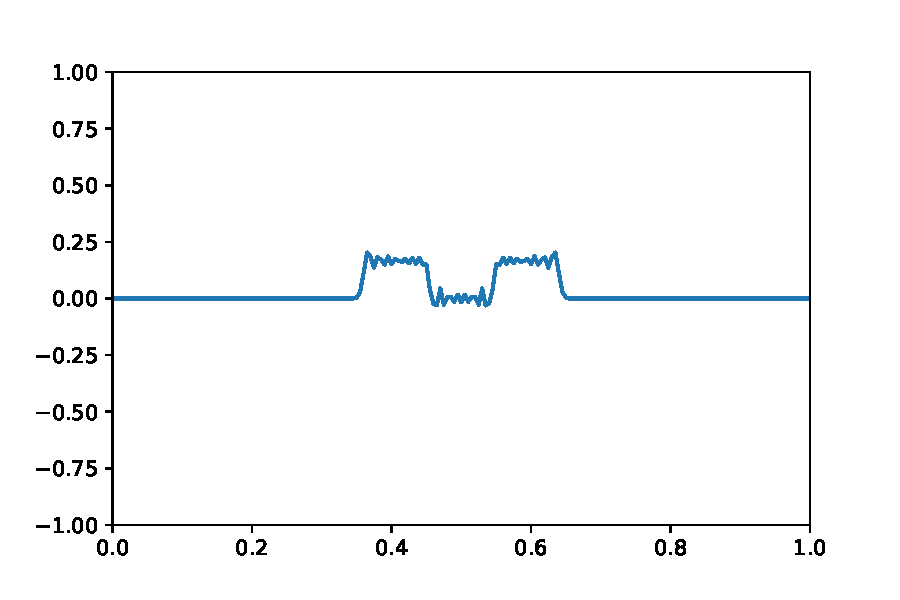
\includegraphics[width=\linewidth]{prob4_t1.pdf}
\caption{$u(x,t = .1)$.}
\end{subfigure}
\caption{The graphs for Problem \ref{prob:prob4} at various times $t$.}
\label{fig:prob4}
\end{figure}
\end{problem}

\section*{Travelling Wave Solutions of an Evolution Equation}
Recall that the advection (transport) equation with initial conditions, given by
\begin{align*}
	&{ }u_t + su_x  = 0, \quad -\infty < x < \infty, \\
	&{ }u(x,0) = f(x),
\end{align*}
has as its general solution $u(x,t) = f(x -st)$.
Consider a general evolutionary PDE of the form
\begin{align}
u_t = G(u,u_x, u_{xx}, \ldots)
\label{evol_pde}
\end{align}
An interesting question to ask is whether \eqref{evol_pde} has travelling wave solutions: is there a signal or wave profile $f(x)$, so that $u(x,t) = f(x-st)$ is a solution of \eqref{evol_pde} that carries the signal at a constant speed $s$?
These travelling waves are often significant physically.
For example, in a PDE modeling insect population dynamics a travelling wave could represent a swarm of locusts; in a PDE describing a combustion process a travelling wave could represent an explosion or detonation.

\subsection*{Burgers' equation}
We will examine the process of studying travelling wave solutions using Burgers' equation, a nonlinear PDE from gas dynamics.
It is given by
\begin{align}
	u_t + \left( \frac{u^2}{2} \right)_x = \nu u_{xx}, \label{eqn:Burgers_pde}
\end{align}
where $u$ and $\nu$ represent the velocity and viscosity of the gas, respectively.
It models both the process of transport with the nonlinear advection term $(u^2/2)_x = u u_x$, as well as diffusion due to the viscosity of the gas ($\nu u_{xx}$).

Let us look for a travelling wave solution $u(x,t) = \hat{u}(x-st)$ for Burgers equation.
We transform \eqref{eqn:Burgers_pde} into the moving frame $(x,t) \to (\bar{x},\bar{t}) = (x-st, t)$. In this frame \eqref{eqn:Burgers_pde} becomes
\begin{align}
	u_{\bar{t}} - s u_{\bar{x}}+ \left(\frac{u^2}{2} \right)_{\bar{x}} = \nu u_{\bar{x}\bar{x}}
	\label{eqn:Burgers_pde_moving_frame}
\end{align}

This new frame of reference corresponds to an observer moving along with the wave, so that the wave appears stationary as the observer studies it.
Thus, $\hat{u}_{\bar{t}} = 0$, so that the wave profile $\hat{u}$ satisfies the ordinary differential equation
\begin{align}
	 -s u_{\bar{x}}+ \left(\frac{u^2}{2} \right)_{\bar{x}} = \nu u_{\bar{x}\bar{x}}.
	\label{eqn:Burgers_ode}
\end{align}

From here on we will drop the bar notation for simplicity.
We seek a travelling wave solution with asymptotically constant boundary conditions; that is,  $\lim_{x \to \pm \infty}\hat{u}(x) = u_{\pm}$

both exist, and  $\lim_{x \to \pm \infty} \hat{u}'(x) = 0$.
We will suppose that $u_- > u_+ > 0$.

Note that to this point we still don't know the speed of the travelling wave.
Integrating both sides of this differential equation, and then taking the limit as $x \to +\infty$, we obtain
\begin{align*}
-s\int_{-\infty}^x u' + \int_{-\infty}^x \left(\frac{u^2}{2}\right)' &= \nu \int_{-\infty}^x u'',\\
-s(u(x) - u_-) + \frac{u^2(x)}{2} - \frac{u_-^2}{2} &= \nu (u'(x) - u'(-\infty)), \\
-s(u_+ - u_-) + \frac{u_+^2}{2} - \frac{u_-^2}{2} &= 0.
\end{align*}
Thus given boundary conditions $u_{\pm}$ at $\pm \infty$, the speed of the travelling wave must be $s = \frac{u_- + u_+}{2}$.

Usually at this point, the travelling wave must be numerically solved using the profile ODE (\eqref{eqn:Burgers_ode} for Burgers equation).
However, the profile ODE for Burgers is simple enough that it is possible to obtain an analytic solution.
The travelling wave is  given by

\[\hat{u}(x) = s - a \tanh \left(\frac{ax }{2\nu} + \delta\right)\]
where $a = (u_- - u_+)/2$ and $\delta$ is fixed real number.
We get a family of solutions because any translation of a travelling wave solution is also a travelling wave solution.

\subsection*{Stability of travelling waves}
Suppose that an evolutionary PDE
\begin{align}
u_t = G(u,u_x, u_{xx}, \ldots).
\label{eqn:evol_pde_repeat}
\end{align}
has a travelling wave solution $u(x,t) = \hat{u}(x-st)$.
An interesting question to consider is whether the mathematical solution, $\hat{u}$, has a physical analogue.
In other words, does the travelling wave show up in real life?
This question is the start of the mathematical study of stability of travelling waves.

We begin by translating \eqref{eqn:evol_pde_repeat} into the moving frame $(x,t) \to (\bar{x},\bar{t}) = (x-st, t)$.
In this frame the PDE becomes
\begin{align*}
u_t - su_x = G(u,u_x, u_{xx}, \ldots).
\end{align*}
In these coordinates the travelling wave is stationary.
Thus, the solution of
\begin{align*}
\begin{split}
u_t - su_x &= G(u,u_x, u_{xx}, \ldots), \\
u(x,t = 0) &= \hat{u}(x),
\end{split}
\end{align*}
is given by $u(x,t) = \hat{u}(x)$.
We say that the travelling wave $\hat{u}$ is asymptotically orbitally stable if whenever $v(x)$ is a small perturbation of $\hat{u}(x)$, the general solution of
\begin{align*}
\begin{split}
u_t - su_x &= G(u,u_x, u_{xx}, \ldots), \\
u(x,t = 0) &= v(x),
\end{split}
\end{align*}
converges to some translation of $\hat{u}$ as $t \to \infty$.
Using this definition to prove stability of a travelling wave is a nontrivial task.

\subsection*{Visualizing stability of the travelling wave solution of Burgers' equation}
The travelling wave solution of Burgers' equation is a stable wave.
To view this numerically, we discretize the PDE
\[u_t -su_x + uu_x = u_{xx}\]
using the second order centered approximations
\begin{align*}
&{ } D_t U_j^{n+1/2} = \frac{U_j^{n+1}-U_j^n}{\triangle t}, \quad
D_{xx}U_j^{n+1/2} = \frac{1}{2} \left( \frac{U_{j+1}^{n+1}-U_{j-1}^{n+1}}{2 \triangle x} +  \frac{U_{j+1}^{n}-U_{j-1}^{n}}{2 \triangle x}\right),\\
&{ } D_{xx}U_j^{n+1/2} = \frac{1}{2} \left( \frac{U_{j+1}^{n+1}- U_{j}^{n+1}+U_{j-1}^{n+1}}{(\triangle x)^2} + \frac{U_{j+1}^{n}- U_{j}^{n}+U_{j-1}^{n}}{(\triangle x)^2}\right)
\end{align*}

Substituting these expressions into the PDE we obtain a second-order, implicit Crank-Nicolson method
\begin{align*}
U_j^{n+1} - U_j^n &= K_1 \big[(s - U_j^{n+1})(U_{j+1}^{n+1} - U_{j-1}^{n+1})
+ (s - U_j^n) (U_{j+1}^n - U_{j-1}^n) \big] \\
&{ }  \quad
+ K_2 \big[(U_{j+1}^{n+1} - 2U_j^{n+1}+ U_{j-1}^{n+1}) + (U_{j+1}^n -2U_j^n + U_{j-1}^n) \big],\\
&{ }  \quad
\end{align*}
where $K_1 = \frac{ \triangle t }{4 \triangle x}$ and $K_2 = \frac{ \triangle t}{2(\triangle x)^2}$.

\begin{problem}
\label{prob:prob5}
Numerically solve the initial value problem
\begin{align*}
	&{ } u_t -su_x + uu_x = u_{xx}, \quad x \in (-\infty,\infty),\\
	&{ } u(x,0) = v(x),
\end{align*}
for $t \in [0,1]$.
Let the perturbation $v(x)$ be given by
\[v(x) = 3.5(\sin{(3x)} + 1)\frac{1}{\sqrt{2\pi}} \exp{(-x^2/2)}\]
And let the initial condition be $u(x, 0) = \hat{u}(x) + v(x)$
Approximate the $x$ domain,$(-\infty, \infty)$, numerically by the finite interval $[-20,20]$, and fix $u(-20) = u_-$, $u(20) = u_+$. Let $u_- = 5$, $u_+ = 1$.
Use 150 intervals in space and 350 steps in time.
Animate your results.
You should see the solution converge to a translate of the travelling wave $\hat{u}$.
See Figure \ref{fig:prob5}.

Hint: This difference scheme is no longer a linear equation.
We have a nonlinear equation in $U^{n+1}$.
We can still solve this function using Newton's method or some other similar solver.
In this case, use \li{scipy.optimize.fsolve}.

\begin{figure}[H]
\centering
\begin{subfigure}{.49\textwidth}
\centering
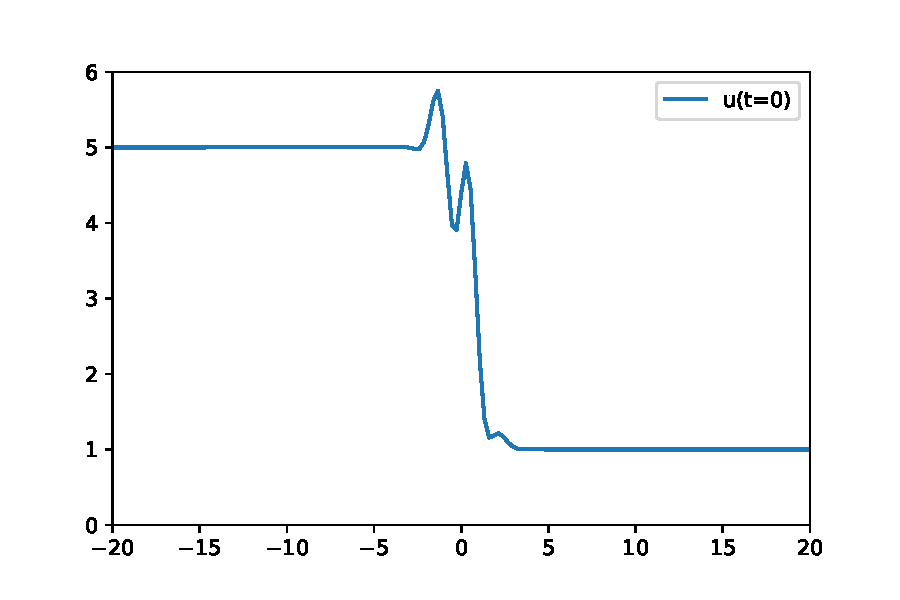
\includegraphics[width=\linewidth]{prob5_initial.pdf}
\caption{$u(x,t=0)$.}
\end{subfigure}
%
\begin{subfigure}{.49\textwidth}
\centering
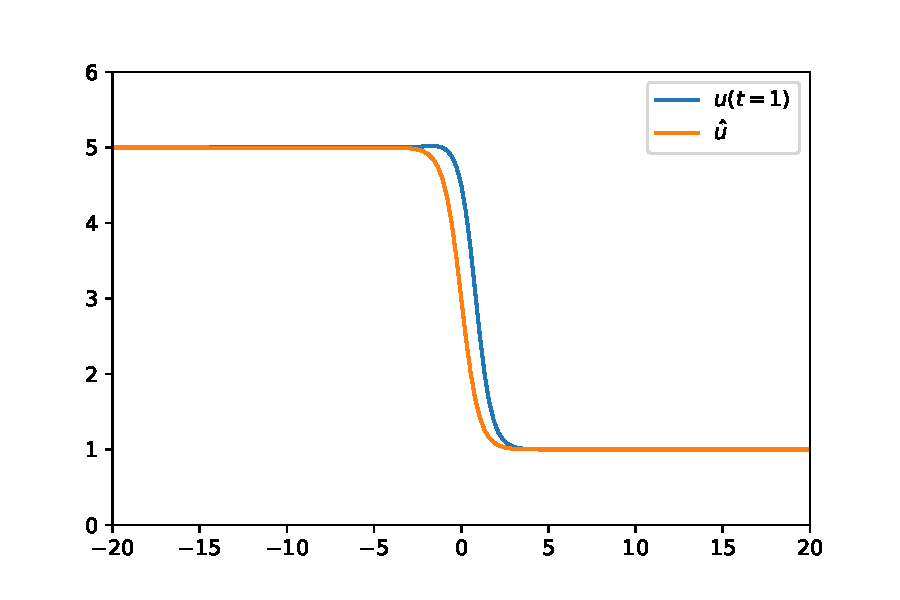
\includegraphics[width=\linewidth]{prob5_ufinal_utilda.pdf}
\caption{$u(x,t = 1)$ vs $\hat{u}$.}
\end{subfigure}
\caption{The graphs for Problem \ref{prob:prob5}}
\label{fig:prob5}
\end{figure}
\end{problem}